\documentclass[11pt,a4paper]{article}

\usepackage[utf8]{inputenc}
\usepackage[T1]{fontenc}
\usepackage[brazil]{babel}
\usepackage[margin=2.5cm]{geometry}
\usepackage{lmodern}
\usepackage{microtype}
\usepackage{xcolor}
\usepackage{tcolorbox}
\usepackage{booktabs}
\usepackage{longtable}
\usepackage{array}
\usepackage{graphicx}
\usepackage{fancyhdr}
\usepackage{parskip}
\usepackage[hidelinks]{hyperref}

% Cores do box de destaque
\definecolor{boxdestaque}{RGB}{242, 244, 248}
\definecolor{boxborda}{RGB}{46, 74, 140}

% ---------------------------------- Cabeçalho e rodapé
\pagestyle{fancy}
\fancyhf{}
\fancyhead[L]{\small REVISÃO CIENTÍFICA: ATAQUES E DEFESAS EM APRENDIZADO FEDERADO}
\fancyfoot[C]{\small Documento de Revisão Bibliográfica - Aprendizado Federado Confiável}
\fancyfoot[R]{\small Página \thepage}
\renewcommand{\headrulewidth}{0.4pt}

\begin{document}

% ---------------------------------- Título
\begin{center}
  {\LARGE \bfseries Revisão de Literatura: Ataques e Defesas em\\[0.3em] Aprendizado Federado}

  \vspace{0.8em}

  {\large \itshape Uma análise sistemática de robustez bizantina, envenenamento e explicabilidade sob\\[0.3em] heterogeneidade de dados}

  \vspace{0.6em}
  \rule{\textwidth}{0.8pt}
  \vspace{1.2em}
\end{center}

% ---------------------------------- Resumo / Introdução
O Aprendizado Federado (FL) emergiu como um paradigma proeminente de aprendizado de máquina colaborativo, permitindo que múltiplos participantes treinem um modelo global de alta qualidade sem compartilhar diretamente seus dados privados. No entanto, por projeto, o FL apresenta vulnerabilidades significativas a ataques adversários na fase de treinamento, como ataques bizantinos, envenenamento de modelo (\emph{model poisoning}), envenenamento de dados (\emph{data poisoning}) e inserção de \emph{backdoors}. Esta revisão de literatura apresenta uma análise robusta e sistemática de dezesseis trabalhos acadêmicos fundamentais, mapeando seus objetivos, ameaças investigadas e mecanismos de defesa propostos para mitigar vulnerabilidades e garantir a segurança e confiabilidade das redes federadas.

\vspace{1.2em}

% ---------------------------- Box de destaque
\begin{tcolorbox}[colback=boxdestaque, colframe=boxborda, boxrule=0.8pt, arc=2pt, left=0.6cm, right=0.6cm, top=0.8em, bottom=0.8em]
\textbf{Especial Atenção à Heterogeneidade de Dados (não-IID):} Muitos dos esquemas clássicos de agregação robusta (AGRs), como Krum e Mediana, foram originalmente projetados sob a premissa de que os dados são distribuídos de forma independente e identicamente distribuída (IID). Trabalhos contemporâneos demonstram que em cenários realistas de \emph{label skewness} (distorção de classes), essas AGRs sofrem severamente com viés de seleção e perdem eficácia de filtragem, motivando o desenvolvimento de defesas adaptativas com dados auxiliares ou aprendizado generativo.
\end{tcolorbox}

\section{Benchmarks de Segurança e Revisões Sistemáticas}
Para estruturar o estudo de segurança em redes federadas, a literatura foca no desenvolvimento de taxonomias de ameaças e ambientes padronizados de teste (\emph{benchmarks}). Cunha Neto et al. (2023) fornecem uma pesquisa abrangente mapeando as vulnerabilidades de FL em duas grandes frentes: ataques à performance do modelo (envenenamento de dados e modelo) e ataques à privacidade dos dados (inversão de modelo e reconstrução via redes generativas adversárias). A pesquisa destaca o papel da criptografia homomórfica e da privacidade diferencial local (LDP) como soluções para proteger os gradientes contra servidores não confiáveis, além do uso de médias geométricas como o RFA para combater o envenenamento de modelo.

Em paralelo, Tariq et al. (2024) estruturam o conceito de Aprendizado Federado Confiável (Trustworthy FL) ao proporem uma arquitetura baseada em cinco pilares fundamentais: Explicabilidade, Transparência, Privacidade/Robustez, Imparcialidade e Responsabilidade (Accountability). Os autores revisam as defesas de agregação robusta e os sistemas de reputação que auxiliam a seleção justa de clientes e distribuição equitativa de recompensas.

No âmbito prático de ferramentas, o \emph{benchmark} Blades (Li et al., 2024) e a biblioteca FedSecurity (Han et al., 2023) fornecem suítes unificadas para simular ameaças. O Blades demonstra empiricamente que as garantias de robustez de AGRs clássicas (como Krum, Median e DnC) são frequentemente superestimadas ao saírem do algoritmo simples FedSGD e operarem sob o amplamente adotado FedAvg com múltiplos passos de atualizações locais (\emph{local epochs}). O FedSecurity (integrado à biblioteca FedML) estende o \emph{benchmarking} para modelos de grande porte (LLMs federados), fornecendo uma arquitetura modular em três níveis (antes, durante e após a agregação) para testar ataques complexos como substituição de modelo e \emph{backdoors} distributivos.

\section{Regras de Agregação Robusta (AGRs) Adaptativas}
As AGRs clássicas enfrentam falhas graves ao lidarem com dados heterogêneos não-IID. Bao et al. (2024) propõem o algoritmo BOBA (Byzantine-Robust and Unbiased Aggregator) para mitigar especificamente os problemas de \emph{label skewness} severa. Os autores provam que as AGRs clássicas sofrem de viés de seleção (degradando classes desbalanceadas) e maior vulnerabilidade bizantina devido ao aumento natural da variação dos gradientes benignos. O BOBA opera em dois estágios: primeiro, projeta os gradientes recebidos em um subespaço de baixa dimensão honesto estimado via Decomposição em Valores Singulares truncada (TrSVD); segundo, usa uma pequena fração de dados no servidor para reconstruir e estimar as classes de cada cliente, filtrando aqueles com coeficientes negativos aberrantes, garantindo convergência ótima.

Outra limitação crítica das AGRs baseadas em distância Euclidiana clássica é a maldição da dimensionalidade em redes profundas. O trabalho Multi-metrics (2023) da SCUT \& Johns Hopkins argumenta que em dimensões elevadas a distância Euclidiana se torna insignificante, permitindo que ataques furtivos como Edge-Case PGD injetem \emph{backdoors} indetectáveis. Para solucionar isso, propõe-se uma filtragem multi-métrica dinâmica que combina as distâncias de Manhattan, Euclidiana e a similaridade de cosseno. O método aplica um processo de branqueamento (\emph{whitening}) para normalizar a variância das métricas sob distribuições não-IID, o que reduz o sucesso de \emph{backdoors} de 55,1\% para 3\% sem comprometer a acurácia da tarefa principal.

No contexto de defesas dinâmicas, Rodríguez-Barroso et al. (2022) desenvolveram o DDaBA (Dynamic Defense against Byzantine Attacks), que ordena e atribui pesos às atualizações dos clientes baseando-se em sua acurácia frente a um conjunto de validação no servidor através de operadores linguísticos dinâmicos. Reconhecendo as fraquezas do DDaBA --- a necessidade de rodadas de aquecimento (\emph{warm-up}) e a propensão a excluir injustamente clientes benignos com dados pobres ---, os mesmos autores propuseram o XI-DDaBA (2024). O XI-DDaBA introduz Explicações Lineares Locais (LLEs) baseadas em mapas de relevância de atributos. Ao invés de avaliar puramente a acurácia, o servidor calcula a similaridade cosseno dos mapas de importância gerados por cada modelo do cliente. Isso garante imunidade a ataques bizantinos desde as primeiras rodadas (sem \emph{warm-up}), além de diferenciar com eficácia atacantes maliciosos de clientes benignos altamente heterogêneos.

\subsection{Resiliência contra Backdoors Furtivos (Ataque Edge-case PGD)}
\textbf{A Falha das Defesas Tradicionais:} Sob o ataque de \emph{backdoor} mais sofisticado e furtivo (Edge-case PGD), as defesas tradicionais falham em proteger o modelo. Agregadores renomados como Krum (59,18\% de sucesso do ataque), Multi-Krum (60,20\%) e RFA (65,31\%) deixam a porta completamente aberta para o invasor.

\textbf{O Sucesso da Abordagem Multi-Métrica:} Ao combinar as distâncias de Manhattan, Euclidiana e similaridade de cosseno com um filtro de ponderação adaptativo, a defesa Multi-Metrics reduz a taxa de sucesso do \emph{backdoor} para meros 3,06\%.

\textbf{Acurácia Preservada:} Diferente do algoritmo Flame (que mitiga o ataque mas reduz a acurácia do modelo global para 81,41\%), a defesa multi-métrica neutraliza o ataque mantendo a acurácia da tarefa principal confirmada em 86,86\%, como ilustrado na Figura~\ref{fig:backdoor}.

\begin{figure}[htbp]
\centering
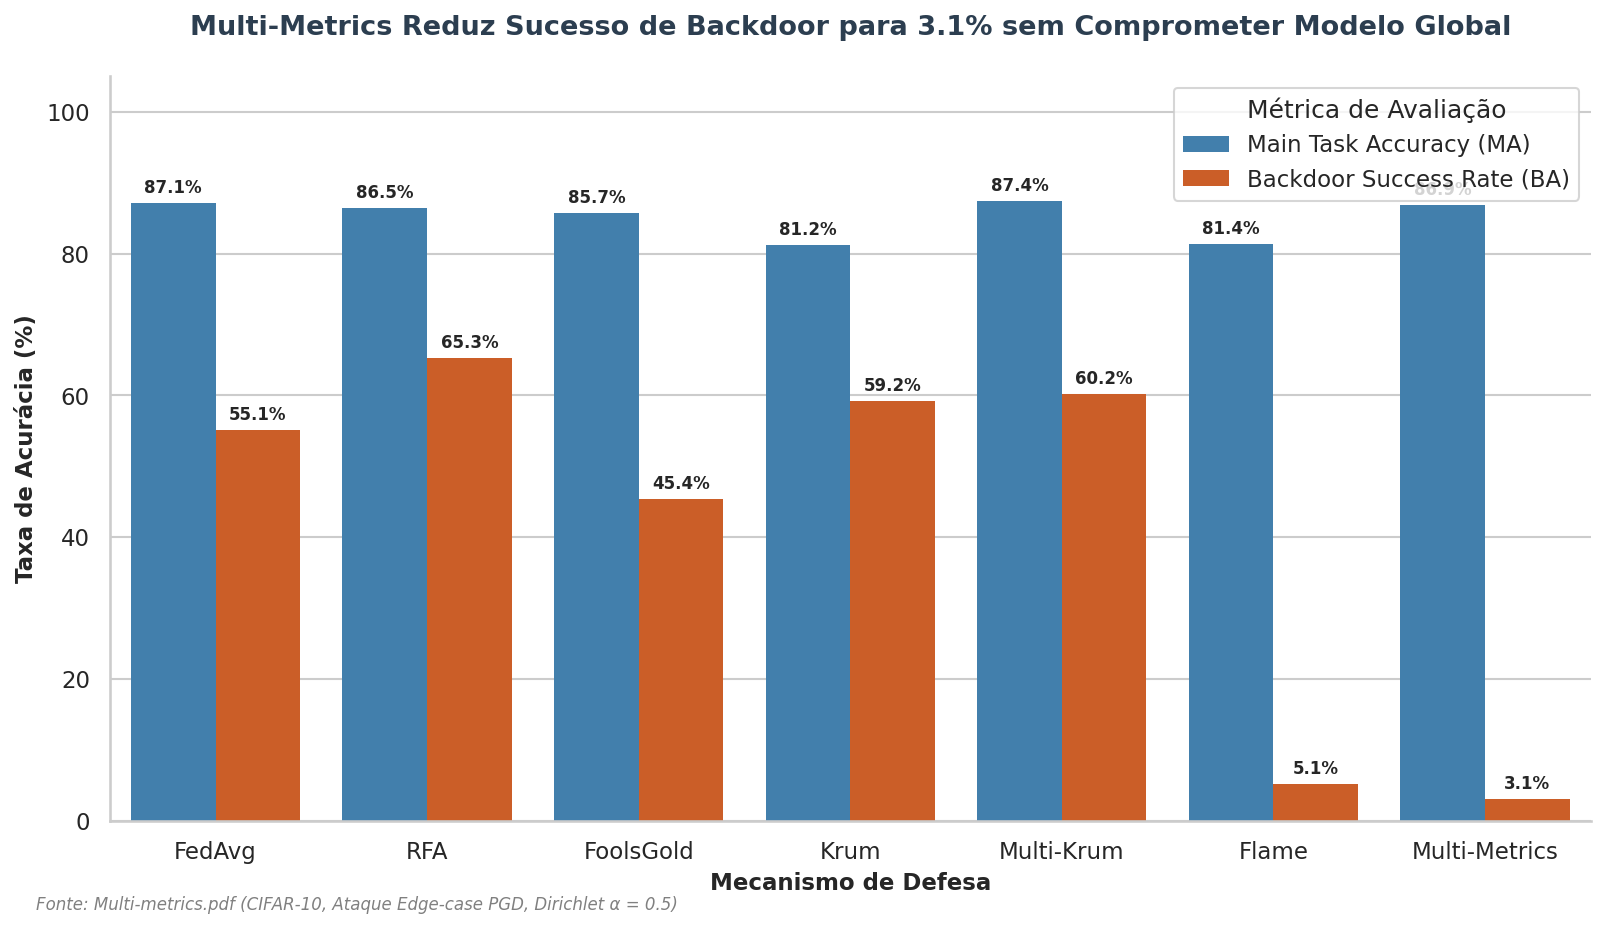
\includegraphics[width=0.85\linewidth]{imagem1_cifar10-backdoor-comparison}
\caption{Comparação de defesas sob ataque \emph{backdoor} Edge-case PGD no CIFAR-10.}
\label{fig:backdoor}
\end{figure}

\subsection{Robustez Bizantina sob Heterogeneidade de Dados (Label Skewness)}
\textbf{A Maldição do Desbalanceamento:} AGRs clássicas assumem dados identicamente distribuídos (IID). Sob condições realistas de \emph{label skewness} (onde clientes possuem dados de poucas classes), o ruído natural dos gradientes benignos confunde as defesas, levando a um colapso completo (com acurácias sob ataque bizantino caindo para 10\% no Average e 14,1\% no Trimmed Mean).

\textbf{A Superioridade do BOBA:} Ao estimar um subespaço honesto via SVD truncado e filtrar anomalias no simplex do servidor, o BOBA alcança 69,2\% de acurácia no pior cenário de ataque bizantino no CIFAR-10. Isso representa um salto de mais de 20 pontos percentuais sobre o segundo melhor \emph{baseline} (FLTrust, com 48,9\%) e mais que o dobro do desempenho do Krum (31,8\%), como ilustrado na Figura~\ref{fig:boba}.

\begin{figure}[htbp]
\centering
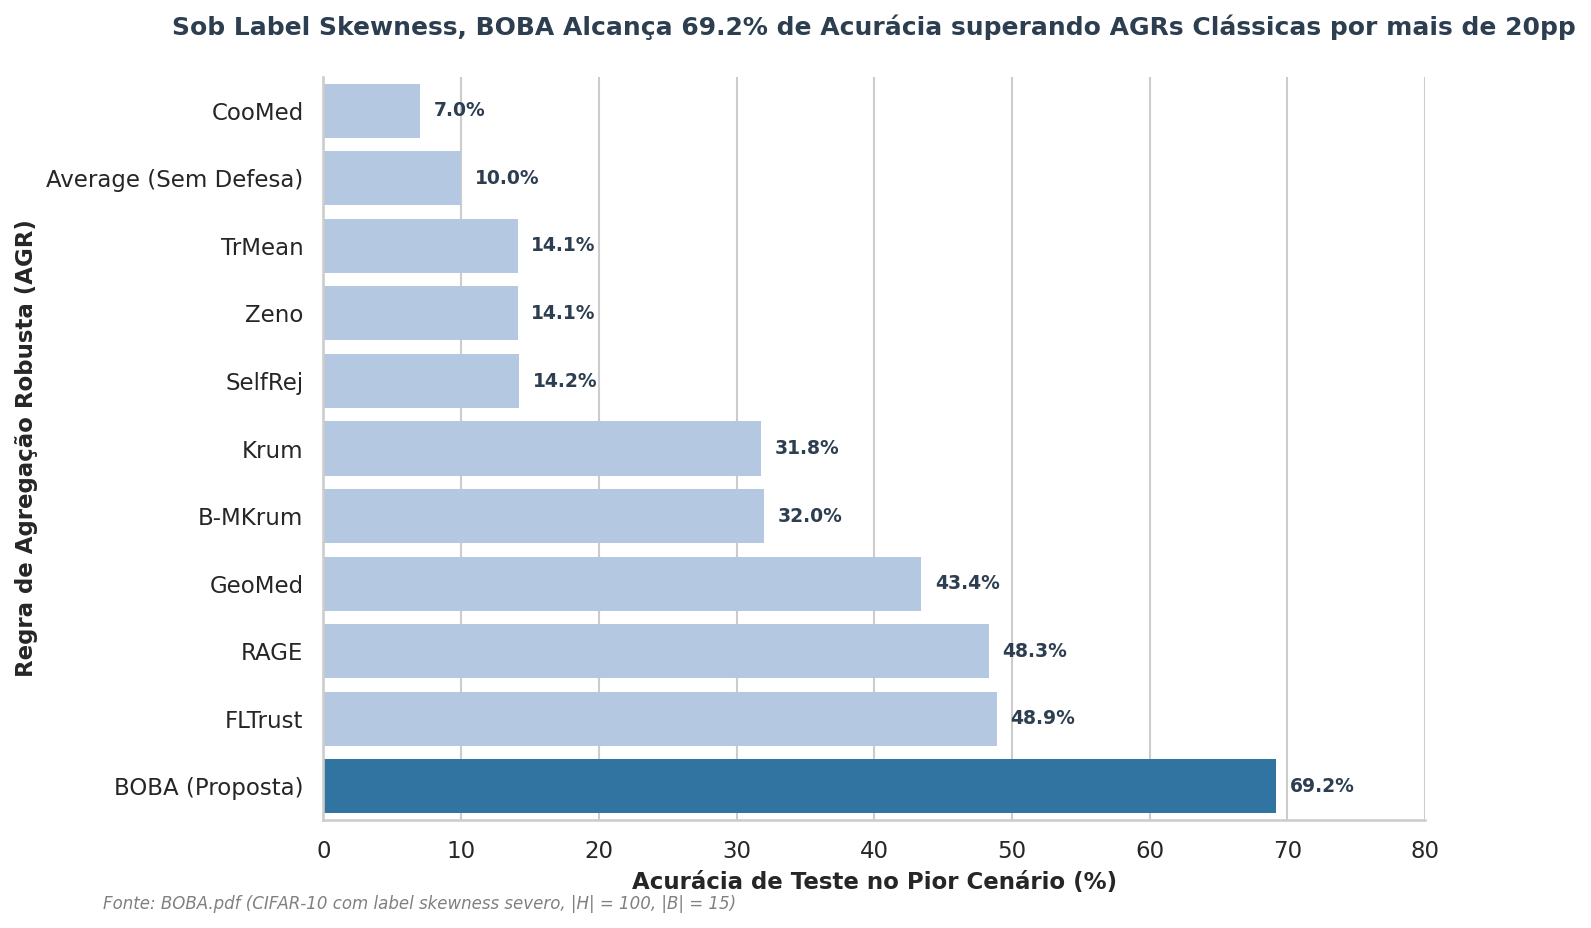
\includegraphics[width=0.85\linewidth]{imagem2_cifar10-boba-byzantine-comparison}
\caption{Comparação entre AGRs sob ataque bizantino em cenários de \emph{label skewness} no CIFAR-10.}
\label{fig:boba}
\end{figure}

\section{Aprendizado Generativo e Abordagens Descentralizadas}
A integração de abordagens generativas visa criar defesas que não dependam de grandes conjuntos de dados externos. O \emph{framework} proposto por Zafar et al. (2024) introduz o uso de uma Rede Adversária Generativa Condicional (cGAN) instalada no servidor. A cGAN é treinada utilizando as fronteiras de decisão do modelo global consolidado para sintetizar amostras de dados artificiais e alinhadas. Esses dados sintéticos são então usados pelo servidor para validar as atualizações de gradientes dos clientes sob três métricas dinâmicas de filtragem (Fixed, Adaptive Mean e Clustered), diferenciando os gradientes bizantinos dos benignos mesmo sob condições severas de não-IID.

Buscando mitigar ataques adaptativos (onde o atacante projeta atualizações maliciosas que mimetizam a direção do gradiente benigno), FLGuard (Karami et al., 2024) desenvolve um sistema baseado em dupla atenção. O FLGuard combina a similaridade cosseno convencional com o erro de reconstrução de gradiente obtido por meio de um Autoencoder Variacional (VAE). Os gradientes dos clientes são passados por um módulo de atenção cruzada e auto-atenção, gerando um escore de confiança dinâmico para cada atualização, evitando filtragens binárias que descartam informações valiosas de nós honestos.

Avançando para ambientes sem infraestrutura centralizada, o algoritmo DF-PAR proposto por Qing et al. (2024) resolve os desafios de aprendizado descentralizado (P2P) aplicado a grades inteligentes de energia (\emph{smart grids}). Cada nó vizinho é avaliado localmente de forma bidimensional (similaridade cosseno e distância de parâmetros). O algoritmo mantém um histórico de credibilidade dinâmico de seus parceiros na grade, mitigando e isolando gradualmente a influência de nós que transmitem gradientes falsificados, mesmo sob ataques sofisticados de inversão de sinal (Converse).

\section{Sensoriamento de Espectro e Ameaças Direcionadas}
No domínio de redes de rádio cognitivo e sensoriamento cooperativo de espectro (CSS), os ataques bizantinos são comumente referidos como Spectrum Sensing Data Falsification (SSDF). Nesse cenário, usuários secundários maliciosos falsificam seus relatórios de energia reportados ao centro de fusão (FC) para induzir erros de ocupação de espectro. Mehmuda et al. propõem um algoritmo de detecção baseado em Isolation Forest. O método analisa o histórico de medições de energia recebido e isola os nós anômalos que desviam substancialmente dos usuários genuínos. De forma análoga, Parmar et al. (2024) abordam o mesmo problema ao propor um algoritmo baseado em Modelos de Mistura de Gaussianas (GMM) treinado pelo algoritmo de Expectação-Maximização (EM). O GMM estima as densidades de probabilidade sob as hipóteses de canal ocupado ou livre, identificando amostras de energia com baixa probabilidade (anomalias). Os autores usam os escores do GMM para determinar pesos adaptativos para cada nó, mitigando completamente a influência de ataques bizantinos probabilísticos (CIPS) sem a necessidade de exclusão binária.

Por fim, a vulnerabilidade estrutural das redes neurais profundas a \emph{backdoors} altamente furtivos é profundamente analisada em Layer-wise Poisoning (Wang et al., 2023). Os autores expõem o conceito de camadas \emph{backdoor}-críticas (BC layers), demonstrando que apenas uma pequena fração de parâmetros (especialmente as primeiras camadas convolucionais e a última camada totalmente conectada) governa o sucesso da inserção do \emph{backdoor}. Ao propor o ataque de envenenamento direcionado a camadas (LP attack) e o ataque de inversão de sinais de camadas (LF attack), eles provam que é possível burlar as AGRs mais modernas (como FLAME, MultiKrum e RLR), pois os gradientes mantêm as propriedades geométricas globais benignas no restante da rede, obtendo altas taxas de sucesso de \emph{backdoor} (BSR) superiores a 90\% em cenários complexos.

Esse cenário de envenenamento de camadas remete às origens das AGRs geométricas como \textbf{Krum} e \textbf{m-Krum} propostas por \textbf{Blanchard et al. (2017)}. Estes métodos fundamentais mostraram que a média ponderada tradicional (FedAvg) é incapaz de tolerar mesmo um único nó bizantino malicioso. O Krum seleciona um único gradiente que minimiza a soma das distâncias Euclidianas quadráticas aos seus vizinhos mais próximos, assumindo que a maioria dos nós é benigna, estabelecendo um limite teórico estrito de tolerância de até um terço de nós maliciosos ($f < n/2 - 1$).

\section{Quadro Comparativo das Obras e Contribuições}
O quadro abaixo consolida de forma concisa e rigorosa os dezesseis trabalhos científicos analisados, estabelecendo uma correspondência clara entre o nome dos artigos, o ano, o evento/veículo de publicação, os ataques analisados e os mecanismos de defesa avaliados.

\vspace{0.8em}

% ---------------------------------- Quadro comparativo (longtable)
\footnotesize
\setlength{\tabcolsep}{3pt}
\setlength{\LTleft}{0pt}
\setlength{\LTright}{0pt}
\begin{longtable}{@{\extracolsep{\fill}} >{\raggedright\arraybackslash}p{2.6cm} >{\raggedright\arraybackslash}p{2.2cm} >{\raggedright\arraybackslash}p{3.9cm} >{\raggedright\arraybackslash}p{2.8cm} >{\raggedright\arraybackslash}p{3.5cm}}
\toprule
\textbf{Artigo} & \textbf{Ano / Evento} & \textbf{Objetivo Central} & \textbf{Ataques Analisados} & \textbf{Defesas Avaliadas} \\
\midrule
\endfirsthead
\toprule
\textbf{Artigo} & \textbf{Ano / Evento} & \textbf{Objetivo Central} & \textbf{Ataques Analisados} & \textbf{Defesas Avaliadas} \\
\midrule
\endhead
\bottomrule
\endlastfoot

BOBA (Bao et al., 2024) & AISTATS 2024 &
Robustez bizantina sob heterogeneidade de dados (\emph{label skewness} severa). &
Gauss, IPM, LIE, Mimic, MinMax, MinSum. &
BOBA (Truncated SVD para subespaço e simplex do servidor). \\ \addlinespace

Blades (Li et al., 2024) & IEEE/ACM IoTDI 2024 &
Suíte de \emph{benchmark} distribuído no Ray para avaliar robustez bizantina realista. &
LabelFlipping, SignFlipping, Gaussian Noise, ALIE, IPM, MinMax. &
Avaliação de AGRs (Median, TrimmedMean, GeoMed, DnC, ClippedClustering). \\ \addlinespace

FedSecurity (Han et al., 2023) & arXiv / FedML &
\emph{Benchmark} de segurança fim-a-fim para FL tradicional e Federated LLMs. &
Byzantine (zero/random/flip), Backdoor, Free Rider, Deep Leakage. &
SLSGD, foolsGold, m-Krum, Bulyan, Norm Clipping, RLR, CRFL. \\ \addlinespace

Survey FL (Cunha Neto et al., 2023) & IEEE Access 2023 &
Pesquisa sistemática PRISMA e taxonomia de ataques à performance e privacidade. &
Model/Data Poisoning, Free-riding, Model Inversion, GAN Reconstruction. &
RFA (geometric median), FoolsGold, PEFL, SMC, LDP (NoPeekNN). \\ \addlinespace

State-of-the-Art FL (Li \& Abdoulmoulah, 2025) & ICCEA 2025 &
Agrupar e classificar esquemas recentes de defesa bizantina em dados heterogêneos. &
Sign Flipping, Gaussian Noise, ALIE, Min-Max. &
FLEST, BOBA, FedSV, FLARM, FLGuard, FPD, DDaBA, FedMP. \\ \addlinespace

GAN-Defense (Zafar et al., 2024) & Uppsala University &
Validar gradientes de clientes usando dados sintéticos de alta fidelidade sem infringir privacidade. &
Random Noise, Sign Flipping, Label-Flipping, IPM. &
Filtros cGAN no servidor (Fixed, Adaptive Mean e Clustered). \\ \addlinespace

FLGuard (Karami et al., 2024) & University of Tehran &
Combater ataques adaptativos mimetizados usando VAE e dupla atenção. &
Scaling, adaptive, label flipping, backdoor attacks. &
FLGuard (VAE para reconstrução de gradiente + atenção dual). \\ \addlinespace

DF-PAR (Qing et al., 2024) & Shenzhen (Conf.) &
Agregação robusta para redes descentralizadas (P2P) de grades inteligentes. &
Little, Gaussian, Random, Converse (inversão de sinal médio). &
DF-PAR (filtragem cosseno-distância + credibilidade histórica). \\ \addlinespace

XI-DDaBA (Rodríguez-Barroso, 2024) & Univ. de Granada &
Garantir imparcialidade para nós benignos e explicar as decisões de filtragem de clientes. &
Label-flipping e envenenamento de modelo (random weights). &
XI-DDaBA (Ponderação dinâmica IOWA baseada em mapas de importância LLE). \\ \addlinespace

Multi-metrics (SCUT / JHU, 2023) & Computer Science Preprint &
Burlar a maldição da dimensionalidade Euclidiana na detecção de \emph{backdoors} de cauda. &
Model replacement, DBA, PGD, Edge-case PGD. &
Agregação multi-métrica dinâmica (Manhattan + Euclidiana + Cosseno + Whitening). \\ \addlinespace

Layer-wise Poisoning (Wang et al., 2023) & arXiv Preprint &
Burlar AGRs baseadas em geometria injetando \emph{backdoors} em camadas críticas (BC layers). &
Layer-wise Poisoning (LP) e Layer-wise Flipping (LF). &
Avaliação de vulnerabilidade em MultiKrum, FLAME, FLTrust, RLR, Flip. \\ \addlinespace

Spectrum Sensing IF (Mehmuda et al., 2023) & SVNIT, Surat &
Detecção de anomalias SSDF em rádio cognitivo usando florestas de isolamento. &
CIPS probabilistic spectrum sensing falsification attacks. &
Isolation Forest aplicado ao histórico de relatórios de energia. \\ \addlinespace

Spectrum CSS GMM (Parmar et al., 2024) & IEEE OJCOMS 2024 &
Combater SSDF em rádio cognitivo via Mistura de Gaussianas e EM. &
CIPS independent probabilistic soft/hard Byzantine attacks. &
GMM com algoritmo EM para detecção de anomalias e atribuição de pesos. \\ \addlinespace

m-Krum / Krum (Blanchard et al., 2017) & NeurIPS 2017 &
Garantir convergência sob ameaças bizantinas arbitrárias no SGD distribuído. &
Vetores bizantinos arbitrários e de conluio coordenado. &
Krum e m-Krum (seleção de modelos baseada em somas de distâncias locais). \\
\end{longtable}

\end{document}
